% Metódy inžinierskej práce

\documentclass[10pt,twoside,slovak,a4paper]{article}

\usepackage[slovak]{babel}
%\usepackage[T1]{fontenc}
\usepackage[IL2]{fontenc} % lepšia sadzba písmena Ľ než v T1
\usepackage[utf8]{inputenc}
\usepackage{graphicx}
\usepackage{url} % príkaz \url na formátovanie URL
\usepackage{hyperref} % odkazy v texte budú aktívne (pri niektorých triedach dokumentov spôsobuje posun textu)

\usepackage{cite}
%\usepackage{times}

\pagestyle{headings}

\title{Používanie serióznych hier na učenie sa jazykov v kontexte írskeho jazyka\thanks{Semestrálny projekt v predmete Metódy inžinierskej práce, ak. rok 2022/23, vedenie: Anna Pylypenko}} % meno a priezvisko vyučujúceho na cvičeniach

\author{Anna Pylypenko\\[2pt]
	{\small Slovenská technická univerzita v Bratislave}\\
	{\small Fakulta informatiky a informačných technológií}\\
	{\small \texttt{xpylypenko@stuba.sk}}
	}




\date{\small 20. september 2022} % upravte



\begin{document}

\maketitle

\begin{abstract}
Myšlienka učiť sa jazyky nielen pomocou učebníc a zošitov je ľuďom blízka už dlho. V oblasti digitálnych vzdelávacích hier sa čoraz väčšej popularite teší digitálne učenie sa jazykov založené na hrách (DGBLL). DGBLL môže poskytnúť študentom príjemný herný zážitok, ako aj zlepšiť ich skúsenosti s učením sa jazykov. Potreba pútavých prístupov k vyučovaniu a učeniu sa menšinových alebo ohrozených jazykov tiež viedla k väčšiemu záujmu o uplatňovanie prístupov DGBLL. V tomto článku sa budem venovať prehľadu hry na učenie írčiny, všetkým výhodám a nevýhodám použitia metódy DGBLL. Keďže tento jazyk patrí medzi ohrozené jazyky, cieľom článku je predpovedať účinnosť tejto metódy učenia sa na zvýšenie záujmu žiakov. Článok sa bude zaoberať témou používania hier ako hlavnej metódy učenia sa jazyka, vytvárania jazykového prostredia prostredníctvom hier, udržiavania záujmu študentov.\\
\quad Keywords: Second Language Acquisition, games and learning, language learning, serious games, Digital Educational Games\\

\paragraph{Môj projekt odpovedá na otázku:}
\begin{itemize}
\item Úvod
\item Koncept hry Cipher: Faoi Gheasa
\item Problém žiakov L1-L2
\item Ako hra rieši tieto problémy? 
\item Výhody a nevýhody používania hier vo vzdelávacom procese
\begin{itemize}
\item Výhody
\begin{itemize}
\item Motivácia
\item Vytvorenie jazykového prostredia
\item Adaptívnosť
\item Chyby sú normálne
\end{itemize}
\item Nevýhody
\begin{itemize}
\item Rovnováha medzi zložitosťou a zrozumiteľnosťou
\item Nedostatok konverzačnej praxe
\item Zložitosť tvorby
\end{itemize}
\end{itemize}
\item Analyz
\item Pracovný postup
\item Záver
\end{itemize}

\end{abstract}


\section{Úvod}

\qquad Írčina je oficiálnym prvým jazykom írskeho štátu, avšak v súčasnosti ňou ako komunitným jazykom hovorí len 3 \% obyvateľstva \cite{BibEntry2020Oct}. Je povinným predmetom v írskych školách, pričom prevažná väčšina detí vo veku od 5 do 18 rokov má denné hodiny jazyka. Napriek týmto významným investíciám
času a prostriedkov, takmer každý tretí tínedžer pri sčítaní obyvateľstva v roku 2011 uviedol, že nevie hovoriť týmto jazykom, a výskum na základných školách ukázal, že od 80. rokov 20. storočia sa prudko znížila úroveň dosiahnutých výsledkov \cite{BibEntry2019Aug}. \\

\section{Koncept hry Cipher: Faoi Gheasa}
\qquad Skupina írskych vývojárov vytvorila hru "Cipher: Faoi Gheasa" na učenie írčiny. Mala by deti zaujímať o učenie sa tohto jazyka a uľahčovať tento proces. Herný svet je magický, v ktorom sa starí zlí duchovia pokúšajú zabrániť prístupu k dávnym mytologickým príbehom tým, že ich zakliali, aby ľudia stratili pamäť na svoju minulosť. Úlohou hráča je rozlúštiť tieto zaklínadlá, aby obnovil príbehy skôr, než budú zapečatené a navždy stratené. K dispozícii je mnoho rôznych kúziel (šifier) a fáz, kým sa podarí zrušiť všetky zlé kúzla a obnoviť príbeh. Hráči zbierajú body, keď správne identifikujú zašifrované slová, a strácajú body, keď sa im nepodarí rozpoznať zašifrované slovo alebo nesprávne identifikujú Faoi Gheasa. Hráči môžu v prípade záujmu použiť svoje body na nákup nápovedy, čo znamená, že hru si môžu užiť aj hráči s minimálnou znalosťou írskeho jazyka. Ak hráč nedokáže nájsť všetky zašifrované slová na stránke, má možnosť "zmeniť koniec" napísaním nejakého textu v írčine, alebo sa pokusu vzdať a v takom prípade sa mu zobrazí tá istá stránka, ale s jednoduchšími šiframi. Hra je vytvorená pomocou Unity (klient) a Photon (server).\cite{Xu2022Jun}\\

\section{Problém žiakov L1-L2}
\qquad Väčšina študentov írčiny, ktorí sa učia ako L2, má angličtinu ako L1. Medzi írčinou a angličtinou existuje mnoho jazykových rozdielov, ktoré môžu vytvárať prekážky pri učení sa írčiny, menšinového jazyka v tieni angličtiny. Jednou z ťažkostí pre L1 používateľov anglického jazyka, ktorí sa učia írčinu, je, že ortografický systém je odlišný od anglického, ale používa rovnakú latinku. Hoci je írsky ortografický systém neprehľadný, je pravidelnejší ako anglický. Pravidlá ortografického systému sa však študenti vo všeobecnosti neučia a často sú odkázaní na to, aby ho dešifrovali sami. Študenti často nevidia zákonitosti, a to im bráni v učení. Automaticky "mapujú" anglický zvukovo-ortografický systém na írsky, čo nie je vždy úspešný prístup. Napríklad slovo teach, ktoré v írčine znamená "dom", sa vyslovuje úplne inak ako slovo "teach" v angličtine. \cite{BibEntry2022May} \\

Ďalším problémom pre študentov írskeho jazyka je, že írčina má zložitý systém počiatočných mutácií. Ide o charakteristický znak keltských jazykov, ktorý ovplyvňuje začiatočné fonémy slovies, podstatných mien, zámen, prídavných mien. Počiatočné mutácie pri podstatných menách sa líšia podľa rodu podstatného mena, t. j. či ide o mužský alebo ženský rod. Na úrovni morfológie sa írske slovesá skloňujú podľa času/spôsobu, osoby a čísla a podstatné mená sa skloňujú podľa čísla a pádu, ktorých tvorenie sa líši podľa rodu podstatného mena.  Študenti írskeho jazyka si často neuvedomujú morfologické a gramatické informácie zakódované v slove, a preto pri snahe porozumieť písanému a hovorenému jazyku strácajú dôležité informácie.\\

 Napríklad v (1) Bhí "was" má počiatočnú mutáciu pre minulý čas, mhór "big" má počiatočnú mutáciu na znak zhody s podstatným menom ženského rodu tine "fire", mbradán "salmon" má počiatočnú mutáciu, pretože je predmetom predložky a určitého člena faoin "under the", a feasa "knowledge" je v genitíve na znak svojho vzťahu k mbradán "salmon".\cite{BibEntry2022May}\\

(1) Bhí tine mhór faoin mbradán feasa. Was fire big under.the salmon knowledge. 'There was a big fire under the salmon of knowledge'\\

\section{Ako hra rieši tieto problémy? }
\qquad V tejto hre tvorcovia podporujú všímanie si pravopisu tým, že do príbehov vkladajú šifrové chyby. Väčšina šifrových chýb nie sú chyby, ktoré by žiak prirodzene urobil, napr. zámena prvej polovice slova s druhou, zdvojenie posledného písmena alebo odstránenie všetkých samohlások. Tieto typy chýb podnecujú k všímavosti, dajú sa pomerne ľahko odhaliť a minimalizujú riziko oboznamovania sa učiacich sa s pravopisnými chybami. Na obrázku 2 majú príklad šifry "Double Tail", ktorá zdvojuje posledné písmeno slova, napr. z Is "is" sa stalo Iss a z mé "me" sa stalo méé.  V tomto experimente tvorcovia podporujú všímanie si rodu podstatných mien, ktorý je ústredným znakom morfosyntaxe írčiny. Používatelia anglického jazyka túto gramatickú vlastnosť írčiny vo všeobecnosti nepoznajú. Tvorcovia to robia ako súčasť rozprávania hry tým, že podstatné mená prezentujú v rôznych farbách v závislosti od ich rodu. Týmto spôsobom tvorcovia uľahčujú všímanie si dvoch odlišných typov podstatných mien. Niektoré zložitejšie šifry odstraňujú farebné označenie podstatných mien a niektoré šifry ovplyvňujú podstatné mená jedného alebo druhého rodu. Preto je v neskorších fázach hry výhodou všímať si a zapamätať si, že jednotlivé slová patria buď k Duchu vody (modré, podstatné mená mužského rodu), alebo k Duchu ohňa (červené, podstatné mená ženského rodu). Na obrázku 2 vidíme, že marúch "morská panna" je červený a dúlachán "temný" je modrý.\\
\section{Prečo je hra lepším spôsobom učenia sa jazyka?} \label{ina}
\qquad Žiaci majú tendenciu používať svoj L1 vo veľkej miere, keď majú menej príležitostí s cieľovým jazykom. Ako uviedli Tomlinson a Masuhara \cite{BibEntry2012Dec} "learners  need  opportunities  to  use language  to  try  to  achieve  communicative  outcomes" .  Na hodinách potrebujú primeranú prax; ukazovať na ceruzku a pýtať sa, čo to je, je úplne neprimerané a vytvára to nudné prostredie na učenie. "Language and activity is an authentic combination for these learners [young learners] – it is one they use in L1" .  Autenticita vnáša do jazykovej triedy záujem a nadšenie.  \\
\qquad Jazyk v hrách je zmysluplný a kontextuálny. Takisto môžeme hry opakovať niekoľkokrát rôznymi spôsobmi a jazyk používaný v hrách je sémanticky zameraný a zmysluplný pre učiacich sa \cite{BibEntry2012Dec} . Hry tiež spájajú formu a funkciu gramatiky v TL (cieľovom jazyku). To znamená, že komunikatívne aspekty jazyka možno dosiahnuť zdôraznením plynulosti aj presnosti. Študenti získajú presnosť aj plynulosť, pretože materiály podobné reálnym, ktoré sú zakomponované v hrách, obsahujú oba tieto prvky. Hry umožňujú žiakom a učiteľom ísť nad rámec tradičných metód a používať naučený jazykový bod v reálnom kontexte. Jazykové hry sú ideálnym nástrojom na to, aby žiaci používali jazyk. Vytvárajú nové výpovede namiesto memorovania fráz. Nielenže si zapamätajú, ako vyplniť prázdne miesta alebo napísať vetu v jednoduchom prítomnom čase, ale aj komunikujú v cieľovom jazyku. Hry teda zvyšujú význam jazyka, pretože práve účasť na jazyku nám umožňuje pochopiť, prečo sa učíme to, čo sa učíme.\\

\section{Výhody a nevýhody používania hier vo vzdelávacom procese} \label{Advantages}
\subsection{Výhody} 
\subsubsection{Motivácia}

\qquad Pre väčšinu detí v základnom veku je jediným kontaktom s írskym jazykom každodenná hodina írčiny, niekoľko fráz v triede v škole a možno náhodné používanie írčiny mimo školy, napríklad v názvoch miest a dopravných značkách. Zatiaľ čo írske deti a dospelí majú tendenciu byť postivielne naklonení jazyku \cite{BibEntry2022Nov}, motivácia môže byť problémom pre deti, ktoré majú obmedzené možnosti používať írčinu mimo školy v autentickej jazykovej komunite \cite{BibEntry2007Oct}. Technológia môže byť kľúčom k spojeniu osôb hovoriacich írskym jazykom s cieľom vytvoriť virtuálnu jazykovú komunitu a vytvoriť prostredie, v ktorom sa írčina používa na komunikáciu zmysluplným a autentickým spôsobom.Hry sú veľmi motivujúce, pretože sú zábavné a zároveň náročné. Okrem toho využívajú zmysluplný a užitočný jazyk v reálnych súvislostiach. \\
\subsubsection{Zníženie úzkosti a stresu} 
\qquad Motivácia, ktorá prichádza s hraním hier, je vo vyučovaní jazykov vysoko cenená, pretože znižuje úzkosť z učenia sa jazyka. Úzkosť je vážny afektívny filter, ktorý stojí v ceste učeniu.  Po vytvorení šťastnej atmosféry v triede budú mať žiaci pozitívny postoj k učeniu sa jazyka. V takomto príjemnom učebnom prostredí sa obmedzí faktor stresu. Vyučovanie jazyka v príjemnej atmosfére prostredníctvom hier umožní kontinuitu učebných aktivít, čo povedie k väčšiemu kontaktu s jazykom. To znamená zvýšený vstup jazyka pre učiacich sa, ktorý je základom pri učení sa aj osvojovaní si jazyka \cite{Cakir2004Sep}.  V kvalitatívnom výskume \cite{Koksal2022Nov} študenti vyjadrili, že ich motivácia pozitívne zvýšila ich nadšenie pre hodiny angličtiny a posilnila ich vnútornú silu. Žiaci sa prostredníctvom hier cítia uvoľnene a nie sú deprimovaní, pretože sa nebudú báť neúspechu. \cite{Akkaya2016Oct}\\

\subsubsection{Vytvorenie jazykového prostredia} 
\qquad Pomocou zaujímavej hry sa jazyk nebude spájať len s nudnými učebnicami a textami. Naopak, dnes už jazyk nie je predmetom v škole, ale nástrojom, pomocou ktorého môžete spoznávať svet na príklade hry. Ľudia budú chcieť vedieť, čo to či ono slovo znamená, pretože sa im bude páčiť príbeh, ktorý prežívajú. Cudzí jazyk bude pre nich kľúčom do tohto sveta.\\

\subsubsection{Adaptívnosť}
\qquad Hra sa ľahko prispôsobí hráčovi. Nemusíte vytvárať knihy rôznych úrovní. Algoritmus to robí za človeka. "Adaptačné prvky v hre sú úroveň obtiažnosti a dĺžka príbehov, ako aj úroveň obtiažnosti a počet kúziel. Hráči sú požiadaní, aby uviedli svoj vek, školský rok a typ školy (anglická alebo írska s vyučovacím jazykom). Dospelí môžu ako svoj vek zadať 18+ a bude im priradená stredná úroveň hry. Podľa počiatočných informácií o používateľovi sa vyberie príbeh, ktorý zodpovedá jazykovým schopnostiam hráča. V priebehu hry sa podľa výkonu hráča upraví úroveň náročnosti a počet kúziel." \cite{Xu2022Jun}\\
\subsubsection{Chyby sú normálne}
\qquad V histórii hry je vždy premyslený moment odoslania hráča. Je dôležité nesústrediť sa na to, aby žiak mohol pokojne pokračovať v hre a nemal pocit, že jeho vedomosti sú malé. "Pri každom dokončení stránky sa môže počet kúziel zvýšiť a kúzla sa stanú náročnejšími. Hráči musia nájsť všetky zakliate slová na stránke a správne určiť použité kúzla, aby mohli postúpiť na ďalšiu stránku príbehu. Ak sa im nepodarí splniť ani jednu z týchto úloh, budú vyzvaní, aby na obrazovke zadali írsku vetu a pokračovali v nedokončenom príbehu (pozri obrázok 1), pričom v takom prípade sa im zobrazí tá istá stránka, ale s inou sadou náhodne vytvorených zaklínadiel. Prípadne môžu príbeh opustiť a zobrazí sa im nový príbeh. "\cite{Xu2022Jun}\\
\subsection{Nevýhody} 
\subsubsection{Rovnováha medzi zložitosťou a zrozumiteľnosťou}
\qquad Napriek mnohým výhodám hier ako učebného nástroja majú hry aj niektoré nevýhody, ktoré treba mať na pamäti, ak sa nepoužívajú správne. Existuje niekoľko bodov, na ktoré by si učitelia mali dať pozor pred použitím hry vo vyučovacom kontexte. Po prvé, musia byť vhodné pre úroveň učiacich sa a cieľ učebnej situácie. Simpson (2011)\cite{BibEntry2022Apr} objasnil, že "vhodnosť sa samozrejme môže týkať mnohých vecí, ako je úroveň náročnosti, zložitosť alebo množstvo času, ktoré spotrebujú v triede" .  Učiteľ má pri aplikácii hry v jazykovej triede obrovskú úlohu. Simpson (2011)\cite{BibEntry2022Apr} varoval pred častým používaním hier. Časté používanie hier môže brániť ich pedagogickej hodnote. Hry sú účinné, keď sa používajú v správnom kontexte a v správnom čase. Neustále používanie hier vyvoláva v žiakoch pocit, že sa nič neučia, preto je pri plánovaní hier kľúčová rovnováha. Žiaci môžu považovať hry len za hry, ale hry sú nabité učením, ak sa praktizujú s vedomím, a preto je príprava hier zvyčajne oveľa časovo náročnejšia ako len vysvetľovanie jazykového bodu.\cite{Akkaya2016Oct}\\

\subsubsection{Nedostatok konverzačnej praxe}
\qquad Hoci hra pomáha pracovať na takmer všetkých zručnostiach: čítanie, písanie, gramatika, počúvanie. Bohužiaľ, nedokáže zabezpečiť bežnú komunikáciu v jazyku. Keďže každý druhý študent má jazykovú bariéru, dôležitým bodom pri osvojovaní si jazyka je nácvik komunikácie.\\

\subsubsection{Zložitosť tvorby}
\qquad Táto hra využíva pedagogickú techniku rozprávania príbehov ako prostriedok učenia sa jazyka. Najlepšími materiálmi na vytvorenie hry môžu byť autentické básne, rozprávky a legendy. Ak však žiadne neexistujú, je lepšie vybrať materiály, ktoré sú pre používateľa zaujímavé. Text by mal byť o jednu úroveň náročnejší, ako sú vedomosti študenta. Nemal by byť príliš zjednodušený. Význam nejasných slov sa dá ľahko nájsť v kontexte. \cite{BibEntry2022May} Hra, ktorú som recenzoval, spĺňa všetky podmienky vzdelávacej hry, pretože využíva aspekty všímavosti \cite{Foster2013Aug}, zvyšovania povedomia, výskumu opravy chýb \cite{Chaudron2006Oct} a zahŕňa prvky z hry s cieľom \cite{BibEntry2008Sep}.

\section{RESULTS OF ANALYZES }
\qquad Táto hra bola testovaná v írskej škole. Žiaci mali možnosť zahrať si hru a potom sa uskutočnil prieskum. Otázky a ich výsledky sú uvedené v nasledujúcej tabuľke. Výsledky týkajúce sa zapojenia študentov do učenia sa írčiny prostredníctvom hry sú sľubné. Pri porovnaní učenia sa alebo čítania írčiny prostredníctvom hry s bežným vyučovaním v triede 73,5 \% účastníkov uviedlo pozitívne odpovede a 73,5 \% účastníkov bolo ochotných hrať hru.\\
\begin{table}
\centering
\begin{tabular}{|c|c|}
\hline
Question &Satisfaction n = 64\\
          &positive (percentage)\\
\hline
Did you like playing the game? &46 (71.9 percent)\\
\hline
What do you think of the storyline in the game? & 38 (59.4 percent)\\
\hline
How willing were you to play the game?& 47 (73.5 percent)\\
\hline
Would you like to play the game more often? &40 (62.6 percent)\\
\hline
What do you think about learning Irish through &40 (62.5 percent)\\
the game? &\\
\hline
How willing were you to read the stories in the&38 (59.4 percent)\\
game?&\\
\hline
How would you compare learning or reading Irish &47 (73.5 percent)\\
through the game to normal classroom teaching?&\\
\hline
How do you feel about learning Irish after playing & 36 (56.3 percent)\\
the game? &\\
\hline
Do you think you learned anything while playing & 33 (51.6 percent)\\
the game? &\\
\hline
What do you think of spells (ciphers) in the game? &44 (68.7 percent)\\
\hline
What do you think of the Irish stories in the game? &39 (60.9 percent)\\
\hline
\end{tabular}
\caption{Proportion of participants’ ratings in terms of gaming experience, learning experience and adaptivity}
\label{tab:corr}
\end{table}
\section{Pracovný postup}
\qquad Na vytvorenie dobrej hry je potrebná interakcia so študentmi počas jej tvorby. Komentáre a testovanie sú rovnako dôležité ako tvorba príbehu hry. Prvou fázou je vytvorenie nápadu a zhromažďovanie materiálov na jeho realizáciu, pochopenie koncepcie hry. Potom je potrebné komunikovať s potenciálnymi používateľmi. Ich želania a návrhy. V druhej fáze, keď je hra vytvorená, sa testuje na školách na žiakoch.\\
\begin{figure*}[tbh]
\centering
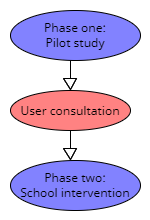
\includegraphics[scale=0.7]{9_diagram.png}
\caption{Pracovný postup}
\label{f:rozhod}
\end{figure*}\\\\

\section{Conclusion} \label{zaver}
\qquad Táto metóda DGRLL je určite vynikajúca na učenie sa jazyka a pomocou hier môžete rozšíriť slovnú zásobu, trénovať počúvanie a písanie. Výhodou počítačových hier je simulácia životných situácií, v ktorých sa hráč môže cítiť ako v reálnom svete. Celý príbeh pomáha vytvárať jazykové prostredie doma. Obrázky pomáhajú nepoužívať slovník. Veľkou výhodou je aj to, že žiak vidí nové neznáme slová v kontexte. To pomáha okamžite si zapamätať, v akej situácii a s akými gramatickými časťami sa slovo používa. Je to užitočné najmä pri jazykoch so zložitou gramatickou štruktúrou. Pri tradičnom učení študenti často zanechávajú výučbu jazykov, pretože neveria vo svoje schopnosti a boja sa veľkého množstva gramatiky. Hra sa však zameriava na plynulé, prirodzené učenie len toho, s čím sa stretávate najčastejšie, t. j. najbežnejších a hlavných konštrukcií. Hra je tiež prispôsobená pre rôzne úrovne hráčov, čo jej dáva výhodu. Írčina je menšinovým jazykom, a tak z toho vyplývajú vyššie uvedené problémy: nedostatok motivácie, materiálov, kvalitných učiteľov a zložitosť gramatiky. Všetky tieto problémy sa riešia vytvorením umelého jazykového prostredia. Inštrukcie by však mali byť jasné a zrozumiteľné, aby sa dosiahol cieľ výučby hry. Hry by mali byť primerané cieľu, pretože nepresný výber hier by narobil viac škody ako úžitku. Počítačové hry sú teda výborným nástrojom na učenie jazykov rôznej náročnosti, ak sú vytvorené metódou DGRLL a používajú sa s mierou. Túto hru a ďalšie podobné hry možno považovať za účinné pri učení ohrozených jazykov. Zistila tiež pozitívnu odozvu od opýtaných študentov. Hlavným aspektom dobrej vzdelávacej hry je proces jej tvorby. Aby bol skutočne účinný, musia sa na jeho tvorbe podieľať skutoční učitelia. Prieskum ukázal, že hra na učenie írčiny má potenciál. Polovici respondentov sa hra páčila, ale potrebuje ďalšie vylepšenia.\\



% týmto sa generuje zoznam literatúry z obsahu súboru literatura.bib podľa toho, na čo sa v článku odkazujete
\bibliography{literatura}
\bibliographystyle{abbrv} % prípadne alpha, abbrv alebo hociktorý iný
\end{document}
